%% josis.tex 1.4   2016-09-15    JoSIS latex template
%------------------------------------------------------------------
% Filename: josis_template.tex
%
% This file is intended as a template for typesetting articles for the
%
%                        Journal of Spatial Information Science.
%
% Please edit this template to generate your own formatted manuscripts
% for submission to JOSIS. See http://josis.org for further details.
%


%%% JOSIS checks in typesetting
%%% * All titles and sections lower case *EXCEPT short title  [ ]
%%% * Remove author postal addresses, only have geographic places and institutions [ ]
%%% * Consistent use of Section, Figure, Table (capitalized and in full) [ ]
%%% * 10 keywords (and all lower case) [ ]
%%% * Remove all avoidable footnotes [ ]
%%% * Use double quotation marks (``'' not "" or `') [ ]
%%% * Punctuation inside quotations [ ]
%%% * E.g. and i.e. followed by comma [ ]
%%% * cf. followed by tilde [ ]
%%% * Itemize and enumerate correctly punctuated [e.g., "1. x, 2. y, and 3. x." ]
%%% * And/or lists using American English punctuation (e.g., "x, y, and z") [ ]
%%% * Bibliography (e.g., en-dashes for number ranges, consistent "Proc.~" for Proceedings of..., etc.) []
%%% * Acknowledgment style use section* [ ]
%%% * et al. no italics, but with dot  [ ]
%%% * All captions end with full stop  [ ]
%%% * Table captions under, not over table  [ ]
%%% * Adjust urls with burlalt [ ]
%%% * Check correct use of hyphens, emdashes, endashes  [ ]
%%% * Perform spell check  [ ]

%%% JOSIS checks directly before publication
%%% Check DOI, page numbers on article and web site. [ ]
%%% Update web site with final title, abstract, keywords. [ ]
%%% Build with distiller for DOI links. [ ]


% Required documentclass definition for JOSIS
\documentclass{josis}
\usepackage{hyperref}
\usepackage[hyphenbreaks]{breakurl}
\usepackage{booktabs}
\usepackage{stmaryrd}
\usepackage[T1]{fontenc}
\usepackage{cite}

% Suggested packages for algorithm formatting
\usepackage{algorithm}
%\usepackage{algorithmic}
\usepackage{algpseudocode}


\usepackage[table]{xcolor}
\usepackage{amssymb,amsmath}

\renewcommand{\topfraction}{0.9}
\renewcommand{\textfraction}{0.1}

% Page setup and overhangs
\sloppy
\widowpenalty=10000
\clubpenalty=10000
\hyphenpenalty=75

% Article details for accepted manuscripts will be added by editorial staff
% Omit year if article in press
% Omit number if article under review
\josisdetails{%
   number=N, year=YYYY, firstpage=xx, lastpage=yy,
  doi={10.5311/JOSIS.YYYY.II.NNN},
   received={December 24, 2015},
   returned={February 25, 2016},
   revised={July 13, 2016},
   accepted={September 5, 2016}, }

\newcommand{\mydoi}[1]{\href{http://dx.doi.org/#1}{doi:\protect\detokenize{#1}}}

%\renewcommand{\UrlLeft}{http:\sslash}
%\DeclareUrlCommand\myurl{\def\UrlLeft{}\def\UrlRight{}%
%\urlstyle{tt}}

\urlstyle{rm}
\makeatletter
% Inspired by http://anti.teamidiot.de/nei/2009/09/latex_url_slash_spacingkerning/
% but slightly less kern and shorter underscore
\let\UrlSpecialsOld\UrlSpecials
\def\UrlSpecials{\UrlSpecialsOld\do\/{\Url@slash}\do\_{\Url@underscore}}%
\def\Url@slash{\@ifnextchar/{\kern-.11em\mathchar47\kern-.2em}%
    {\kern-.0em\mathchar47\kern-.08em\penalty\UrlBigBreakPenalty}}
\def\Url@underscore{\nfss@text{\leavevmode \kern.06em\vbox{\hrule\@width.3em}}}
\makeatother

\hypersetup{
colorlinks=true,
linkcolor=black,
citecolor=black,
urlcolor=black
}

% Add the running author and running title information
\runningauthor{\begin{minipage}{.9\textwidth}\centering Fleischmann, Vybornova\end{minipage}}
\runningtitle{Bananas and tangerines}

% Document begins
\begin{document}
%\setcounter{page}{33}


% Insert your own title
\title{Bananas and tangerines spilled on streets}

% Insert your manuscipts authors, affiliations, and addresses
\author{Martin Fleischmann}\affil{Geographic
Data Science Lab, Department of Geography and Planning, University of
Liverpool, United Kingdom}
\author{Anastassia Vybornova}\affil{NEtworks, Data and Society (NERDS), Computer Science Department, IT University of Copenhagen, Denmark}

\maketitle

% Add 5-10 keywords for every submission
\keywords{street networks, blocks, urban form, shape analysis, urban morphology, urban morphometrics, routing}

% Add a short abstract of 150-250 words
\begin{abstract}
    1-2 sentences basic introduction into field. 2-3 sentences more detailed background. 1 sentence clearly stating the general problem being addressed by this particular study. 1 sentence summarizing the main result (“here we show”). 2-3 sentences explaining what the main result reveals/adds. 1-2 sentences to put results into more general context. Optional - if accessibility is enhanced by this: 2-3 sentences to provide broader perspective.
\end{abstract}

% Your main text begins here.
\section{Introduction}
\label{sec:intro}

\subsection{why do we care?}

1 paragraph general motivation - framework of urban data science. why everyone would benefit from having this issue solved. cite arcaute on 'recent advances, lobo on 'urban science'. also: alessandretti 2020, louail 2015, barthelemy books (morphogenesis 2018; spatial networks 2022)

2-3 sentences morphometrics (fleischmann, porta, dibble, etc.) diet 2018 on planar map classification. sharifi on urban forms.

1 paragraph problem description - cite cardillo, geisberger, morer (computational costs), maybe venerandi 2016?; vanegas paper on actually *simulating* these spaces

1 paragraph examples - other authors complaining about the issue, without having solved it yet (e.g. best paper ever \citep{vybornova2022automated}); grippa 2018; peponis 2007 merges these into urban blocks (replacing by center lines)

1 paragraph summary of what happens in this paper - 'towards an automated detection of bananas';
method inspired by louf and barthelemy;
tried out on X cities across the world,
from different morphological classes (cite fleischmann);
2 sentences about using OSM as data source, and OSMnx/geopandas/momepy (...) for processing;
code is open source (?) ;

Adding some text here.

\section{Method}
\label{sec:method}

Make a strong case for the fact that our method is very simple (it is not a machine learning algorithm); computationally cheap; AND manages to capture BOTH elongated bananas and intersection bananas with ONE stroke and ONE index, which is possible thanks to the CHARACTERISTIC PATTERNS in urban street networks. As demonstrated in the scatter plot \ref{fig:banana-scatter}...

\begin{figure}
    \centering
    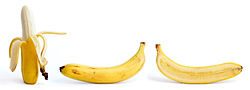
\includegraphics{figures/banana}
    \caption{[Show shape index v. area plot for different continents (?) or for different FUA(s) to show the banana shape in the distribution]}
    \label{fig:banana-scatter}
\end{figure}

% COMMENTING OUT THE NOTES
% - select sample of urban areas (FUA)
% - fetch the data from OSM
% - polygonize the network
% - measure shape charactersitics
%     - TODO: measure initally more than Reock (get a sample from ESDA)
%     - there is a conceptual backbone to this - we know that the artifacts are either
%     small (small intersections) polygons or can be large but then they are very narrow
%     (in between dual carriegaway)
%     - we need a shape metric that captures this relationship
% - identify optimal measurements
%     - plots that help us visually detect a cluster of artifacts
% - derivation of 1-dimensional index
%     - from Roeck and area we can derive one value from which distribution we can
%     identify a cut-off value for artifact/non-artifact polygons
% - cut-off value detection
% - exploration of geographical variation
%     - differences between cities and continents
% - open tools, open data, open code with full reproducibility

\subsection*{Method section on using shape indeces}
mention Sanzana \cite{sanzana_decomposition_2018}, Louf \cite{louf_typology_2014}, ... etc.


\textit{Sanzana et al. propose an algorithm for identification and elimination of ``bad-shaped polygons'', incl. streets/roads/footpaths. Explain that while we have a comparable approach, we are concerned with *cities* while they are concerned with *hydrological models*; and since cities express some certain regularities we can make use of that}

\subsection*{Method section on finding the minimum and using it as a threshold (put part of this in results maybe?)}

\begin{figure}
    \centering
    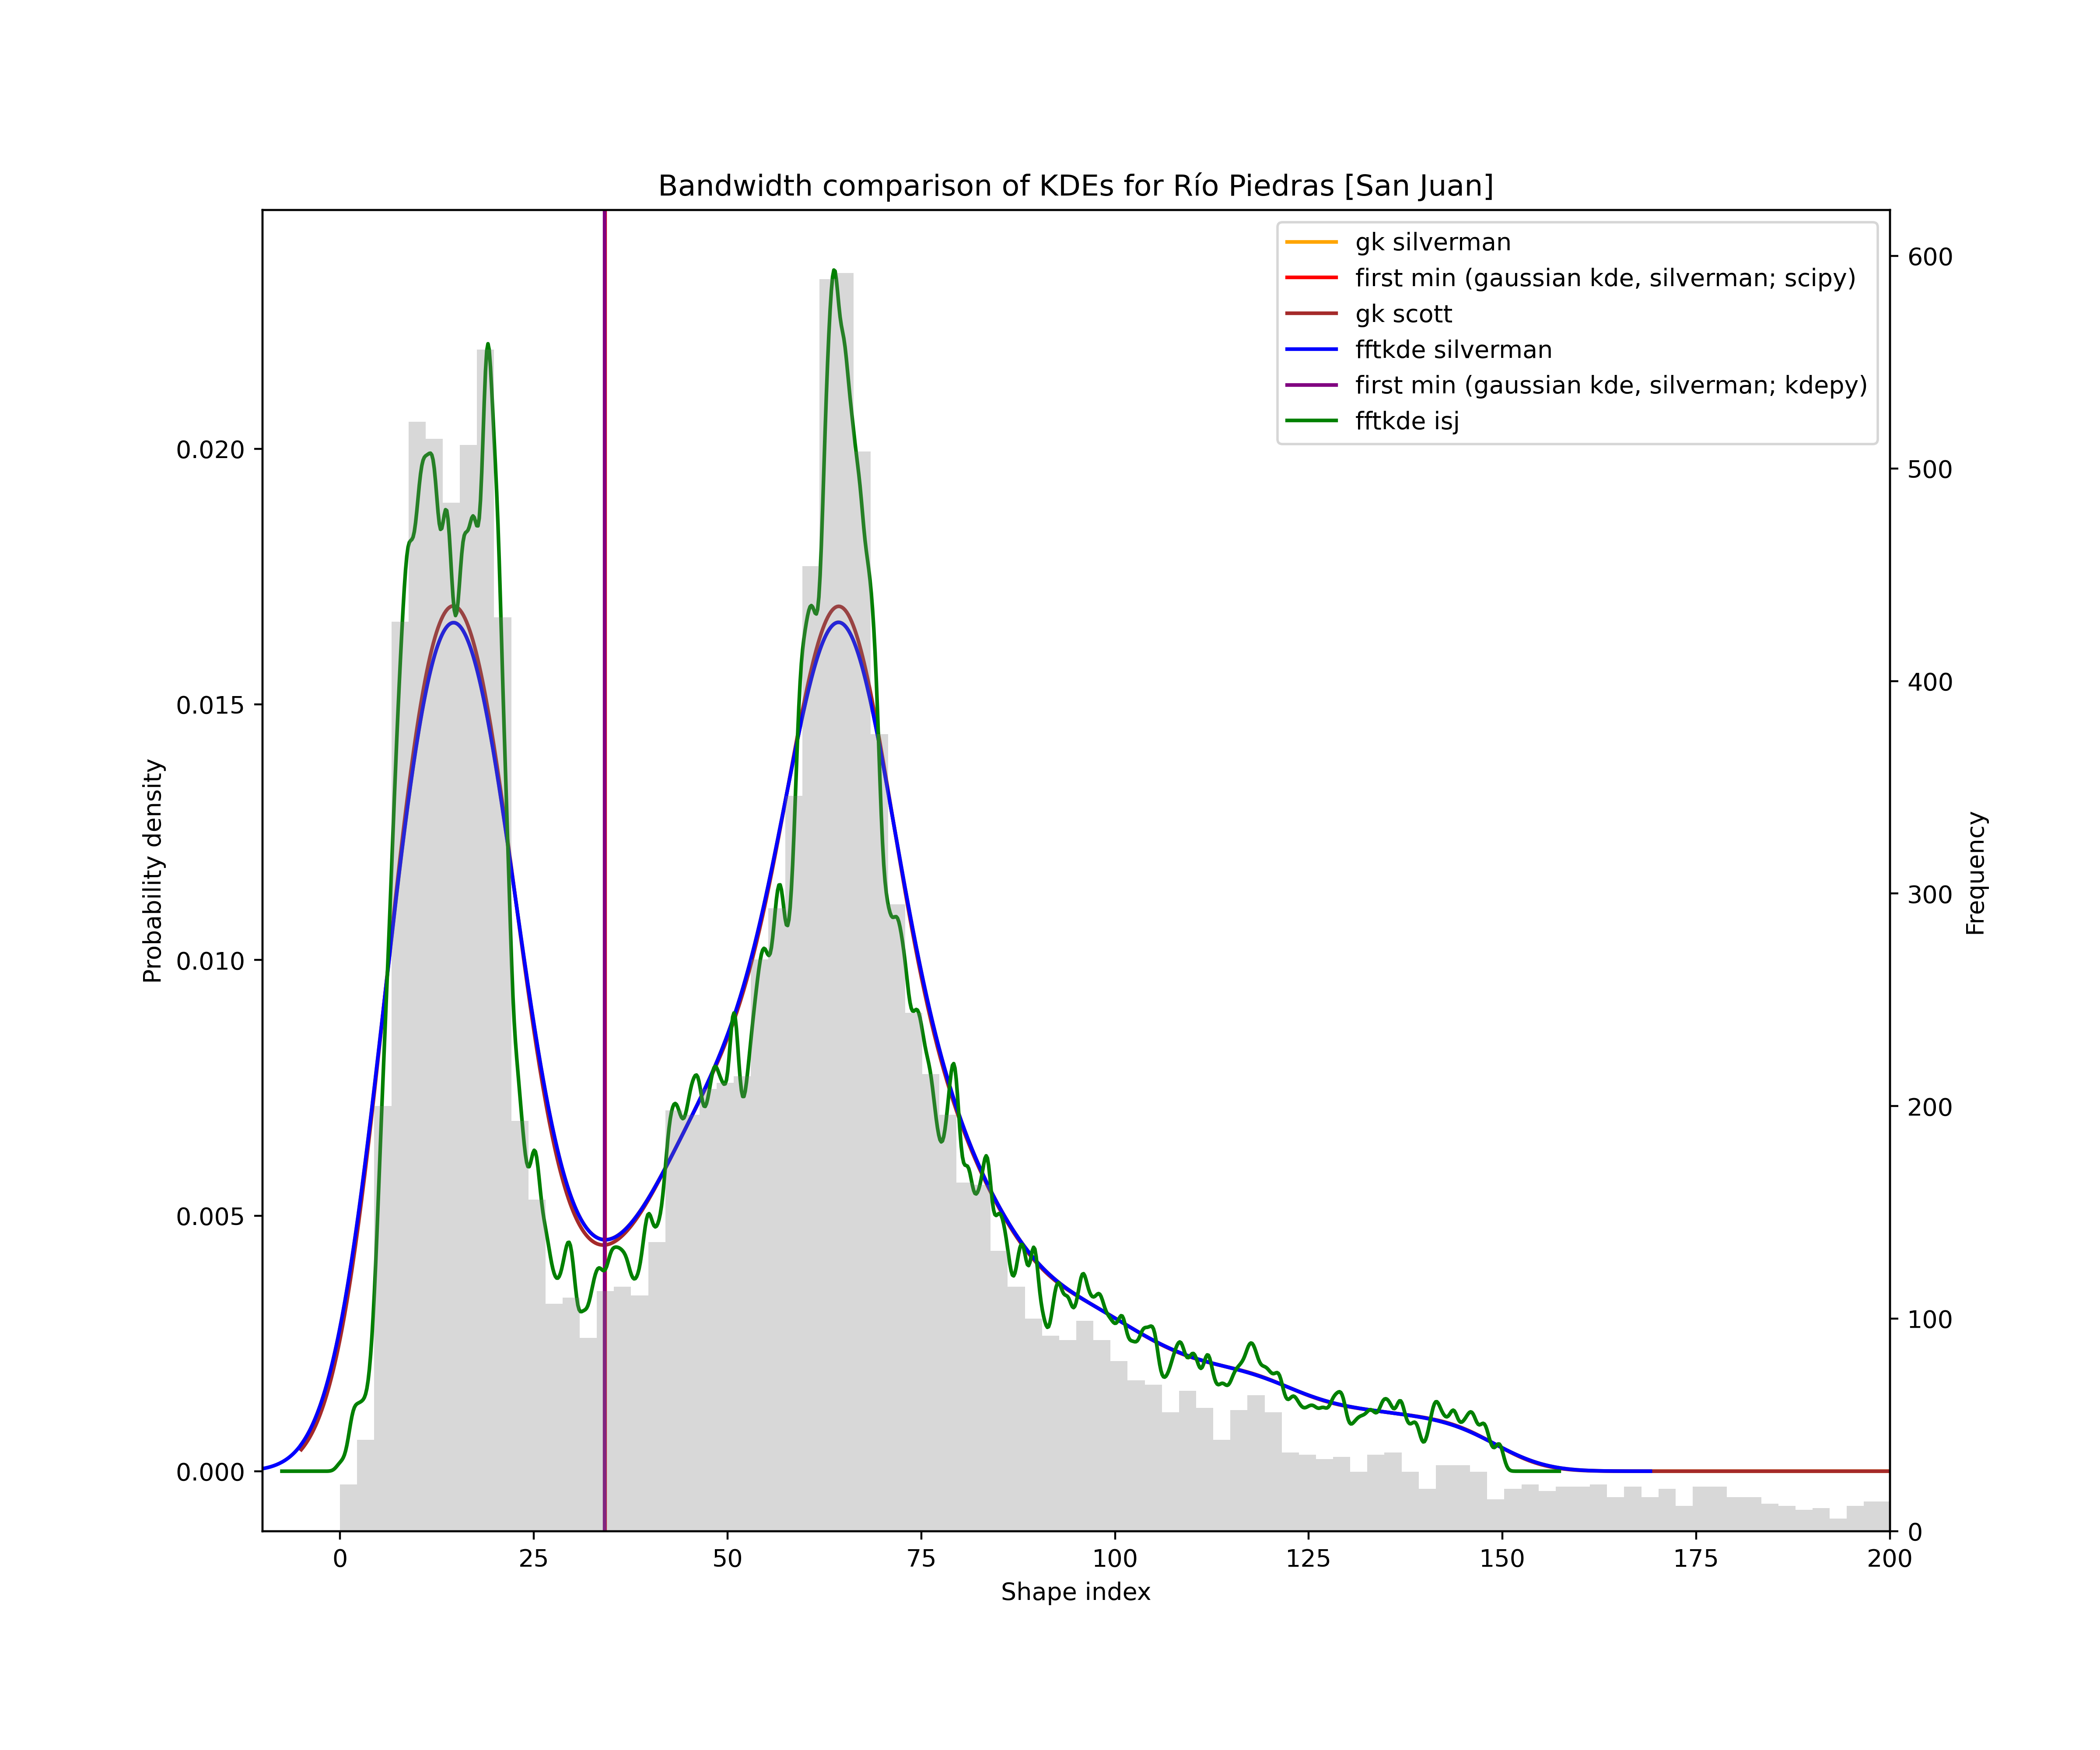
\includegraphics[width=0.5\linewidth]{figures/308}
    \caption{[Above: just a placeholder. Insert here: shape index frequency distribution(s) for FUA X. - show the two-peak pattern]}
    \label{fig:si-dist}
\end{figure}

Many, though not all, shape index frequency distributions for the analyzed FUAs reveal a common feature of two prominent peaks (see Figure \ref{fig:si-dist}). Through visual analysis, we find that these peaks represent two different types of polygons. Most of the polygons from the first (leftmost) peak can be attributed to ``bananas’’ in the street network, whereas most of the polygons from the second (rightmost) peak represent true urban blocks. Therefore, for FUAs that show a pronounced two-peak pattern in their shape index frequency distribution, the minimum \textit{between} the two peaks can be used as shape index threshold: polygons with a shape index below the threshold will most likely be ``bananas’’; polygons with a shape index above the threshold will most likely be true urban blocks. To derive the minimum, we approximate the shape index frequency distribution with a Gaussian kernel density estimation. For bandwidth selection, we use the parametric Silverman method \cite{silverman_using_1981} and find that it gives satisfactory results; non-parametric bandwidth selection methods might be a subject for future work (see section \ref{sec:discussion}). 

Next, comparing the positions of peak 1, peak 2, and shape index threshold for different FUAs with pronounced two-peak patterns, we find that maxima positions vary to a considerably greater extent than minima positions. In other words, shape index thresholds for ``banana’’ identification from morphologically different FUAs lie within a relatively narrow range. We therefore hypothesize that applying a shape index threshold within the range identified from FUAs whose polygons follow a two-peak distribution will allow the identification of ``bananas’’ polygons even for those FUAs whose distributions do not show a two-peak pattern. Applying the … [TBD: lower boundary/median/average/higher boundary] of the empirically derived shape index threshold range to the rest of FUAs indeed reveals ``bananas´´ polygons in all/most FUAs (see Figure \ref{fig:city}).

\section{Results}
\label{sec:results}

- area vs shape plots
    - use all cases together and show multiple shape indices
- Reock as an optimal index (?) [I think it will be the optimal one but we need to verify that]
- 1-dimensional index formula (if we use Reock it is the one from the banana notebook)
- shape-index plots with cut-off values
- plots based on geographical location
    - distributions, Reock-area scatters
    - describe the differences
- formalise the detection workflow


\section{Discussion}
\label{sec:discussion}

How could this be used?

how to move forward? (sneak preview of google summer of code) - the simplification problem can be seen as a problem of the elimination of banana

incorporate further data (ideas: directionality; street names; angles; land use; ...)
use network formalism: on dual approach (intersections = edges): jiang 2004, yang 2022,
rosvall/sneppen; barthelemy paper on shortest path shape

end with a call to action \& 'towards open urban data science'

\bigskip

include in future work:
\begin{itemize}
    \item analyze other regularities in distribution
    \item !! once banana has been found: how to replace it?
    \item non-parametric bandwidth selection
\end{itemize}


% \section{Introduction}

% This template provides a guide to formatting articles for submission to the Journal of Spatial Information Science, JOSIS, \burl{http://josis.org}. When preparing an article for submission, please follow this template closely, referring to past JOSIS articles (open access on the JOSIS web site) for further examples.

% \section{Author guidelines}

% \subsection{Manuscript preparation}
% Manuscripts must be written in English in a clear, direct, and active style. All pages must be numbered sequentially. The manuscript should be submitted as a PDF file based on this \LaTeX template.

% \subsection{Title}
% The title should be concise, and must not be more than 20 words. Authors should also provide a short ``running title.''

% \subsection{Authors and institutional affiliations}
% Authors are required to provide their full names and their institutional affiliations, omitting postal addresses.

% \subsection{Abstract}
% The abstract should summarize the essential features of the article, and must not exceed 250 words for full papers. Abbreviations should be avoided in the abstract, and references should not be cited in the abstract.

% \subsection{Keywords}
% Your submission must include between five and ten keywords for your article. Accepted manuscripts must additionally specify further index terms as appropriate.

% \subsection{Main Text}
% The main text should be divided into separate sections, and may be further subdivided according to the areas to be discussed. The manuscript style must be uniform throughout the text using 11pt Palatino font. The first appearance of any abbreviations in the text should be preceded by the full term, unless it is a standard abbreviation or unit of measurement. Reference numbers should be given in square brackets in the text. Common or assimilated words from Latin or other languages should not be italicized, including per se, et al.

% \subsection{Style}

% Many examples of the journal style can be seen in existing JOSIS published articles, \url{http://josis.org}. Please pay particular attention to the following style requirements:

% \begin{itemize}
% \item Spelling: Please use standard American English spelling throughout.
% \item Punctuation: JOSIS uses standard American English punctuation. In
% particular, please ensure:
% \begin{itemize}
% \item all lists items are always separated by
% punctuation (e.g., ``a, b, and c'' but not ``a, b and c''); and
% \item commas and periods always appear inside quotation marks (e.g., ``x, y, and z.'' but not ``x, y, and z''.).
% \end{itemize}
% \item Capitalization: JOSIS style is to only use capitals only for the
% beginning of sentences, proper nouns, names (e.g., Norman, ArcMap) and,
% where appropriate, acronyms (e.g., GIS). Please avoid capitalization of
% other words (e.g., ``geographic information systems (GIS)'' but not
% ``Geographic Information Systems (GIS)'') and in titles, including section headings (e.g., ``Affordance-based individuation of junctions in Open Street Map" but not ``Affordance-Based Individuation of Junctions in Open Street Map'').
% \end{itemize}


% \subsection{Figures}
% Figures and Tables must be numbered consecutively with a concise explanatory caption, and must be referred to in the main text with capitalized reference (e.g., ``Figure \ref{fig:1}'' or ``Table \ref{tab:1}''). Figures and Tables must appear in the text close to where they are first referred to in the main text. Figure and table captions come below the figure or table. Do not collect figures or tables together at the end of the article. Authors of accepted articles will need to supply high quality versions of all figures as separate .eps (encapsulated postscript) files.

% \begin{figure}[tbh]
% \centering
% \includegraphics[width=\textwidth]{Figure1}
% \caption{An illustrative figure, after \cite{huck15.JOSIS}.}\label{fig:1}
% \end{figure}

% \begin{table}
% \centering
% \begin{tabular}{lrr}
% \hline
% Text column & Numerical column 1 & Numerical column 2\\
% \hline
% First row& 10 & 0.003\\
% Second row& 52& 10.037\\
% Third row& 729 & 150.315\\
% ...& ...& ...\\
% \hline
% \end{tabular}
% \caption{Example table with preferred line rules and alignment.}\label{tab:1}
% \end{table}

% \subsection{Algorithms}

% Algorithms should be formatted using standard algorithm packages where possible, as in Algorithm~\ref{alg:1}.

% \begin{algorithm}[htb]
% \caption{Example algorithm formatting after \cite{zhong16.IJGIS}} \label{alg:1}
% \footnotesize
% \begin{algorithmic} [1]                   % enter the algorithmic environment
% \Require A finite set of two-dimensional points $P \subset \mathbb{R} \times \mathbb{R}$ and one parameter $\lambda \in \mathbb{R}$
% \State Construct the Delaunay triangulation $DT(P)$ of $P$
% \State $\Delta \gets DT(P)$
% \State Construct the list $B$ of exterior edges of $DT(P)$
% \State Sort the list $B$ in descending order of edge length
% \State Initialize the $v\!-\!boundary$ function
% \State Set the root ($r$) of $\mathbf{T}_{{\chi}}(P,\, \lambda)$ to be \{edge = $\emptyset$, oppositeVertex = $\emptyset$, length = $\emptyset$\}
% \State Construct the list of parent nodes ($PN$) for the elements in $B$
% \State Set each element in $PN$ to be $r$
% \State $O(P,\, \lambda) \gets \emptyset$
% \While{$B$ is not empty}
% 	\State $e = \{d_1,\, d_2\} \gets$ pop($B$)
% 	\State $p \gets$ pop($PN$)
% 	\State $o \gets$ opposite vertex of $e$ in $\Delta$
% 	\State $N \gets$ \{edge = $e$, oppositeVertex = $o$, length = $||e||$\}
% 	\State Insert $N$ in $\mathbf{T}_{{\chi}}(P,\, \lambda)$ as a child of $p$
% 	\State $node(d_1) \gets N$
% 	\State $node(d_2) \gets N$
% 	\State Append $N$ to $O(P,\, \lambda)$
% 	\If{$||e|| > \lambda$ \textbf{and} $v\!-\!boundary(o) = false$}
% 		\State Remove $e$ from $\Delta$
% 		\State $v\!-\!boundary(o) = true$
% 		\State Insert the arms of $e$ in $\Delta$ into $B$ in order of edge length
% 		\State Insert $N$ into $PN$ at the corresponding position of the arms of $e$ in $B$
% 	\EndIf
% \EndWhile
% \State \textbf{Return} $\chi(P,\, \lambda)$ formed by leaves of $\mathbf{T}_{{\chi}}(P,\, \lambda)$, $DT(P)$, $\mathbf{T}_{{\chi}}(P,\, \lambda)$ and $O(P,\, \lambda)$
% \end{algorithmic}
% \end{algorithm}

% \subsection{Footnotes}
% Footnotes are strongly discouraged in text. Where footnotes must be used, they should be numbered consecutively.


% \section{References}
% References must be listed in the numerical system (ACM). Citations must be numbered sequentially [in square brackets] in the main text. Full numbered references must be listed in the reference section in alphabetical order. The reference numbers must be finalized and the bibliography must be fully formatted before submission. Examples of citation styles included in the bibliography for this document include journal articles \cite{overEtAl2010,arkin}, authored books \cite{bailey}, edited books \cite{miller09.BOOK}, articles in proceedings \cite{champion11}, articles in books or collections \cite{Grosso12}, theses \cite{ruas99}, technical reports \cite{blasertr}, and web resources \cite{web}.

% \subsection{DOIs}

% All JOSIS articles must list the DOI of all references, where a DOI exists, see
% \url{http://josis.org/index.php/josis/about/submissions#authorGuidelines} for examples. Please check carefully to add the DOIs for cited references,
% adding DOIs to all references that have one. DOIs may be added in the ``doi'' field of the bibtex file.

% DOIs can be found via \url{http://www.crossref.org/guestquery/} as well as many
% other search engines and publisher pages (e.g., Scopus, SpringerLink).


% \section{About JOSIS}

% The Journal of Spatial Information Science (JOSIS) is an international, interdisciplinary, open-access journal dedicated to publishing high-quality, original research articles in spatial information science. The journal aims to publish research spanning the theoretical foundations of spatial and geographical information science, through computation with geospatial information, to technologies for geographical information use.

% JOSIS encourages submissions from topics including, but not limited to spatial and spatiotemporal information systems; computational geometry, geocomputation, spatial algorithms; geovisualization, cartography, and geographical user interfaces; computing with spatiotemporal information under uncertainty; spatial cognition and qualitative spatial reasoning; spatial data models and structures; conceptual models of space and geoontology; distributed and parallel spatial computing, web-based GIS, and interoperability; context- and location-aware computing; and applications to GIS, spatial databases, location-based services, geosensor networks, and geosensor web. The journal publishes full-length original research articles, as well as survey-style review papers. In addition, the journal publishes shorter articles in three sections: reports from community activities, letters to the editors, and book reviews.

\section*{Acknowledgments}

% Acknowledgments appear in a separate unnumbered section before the bibliography. Please acknowledge anyone (individual/company/institution) who has contributed to the study, including substantial contributions to the conception, design, acquisition of data; analysis and interpretation of data; drafting the manuscript; or provided critical comments resulting in revisions to content. For each author, please list the source(s) of any funding or financial contributions related to the study.
To be added. Remember to include ESRC/ATI funding covering initial experiments.

\bibliographystyle{josisacm}
\bibliography{refs}

\end{document}